\documentclass{standalone}
\usepackage{tikz}
\usetikzlibrary{patterns, positioning}
\usepackage[sfdefault]{ClearSans} %% option 'sfdefault' activates Clear Sans as the default text font
\usepackage[T1]{fontenc}

\begin{document}
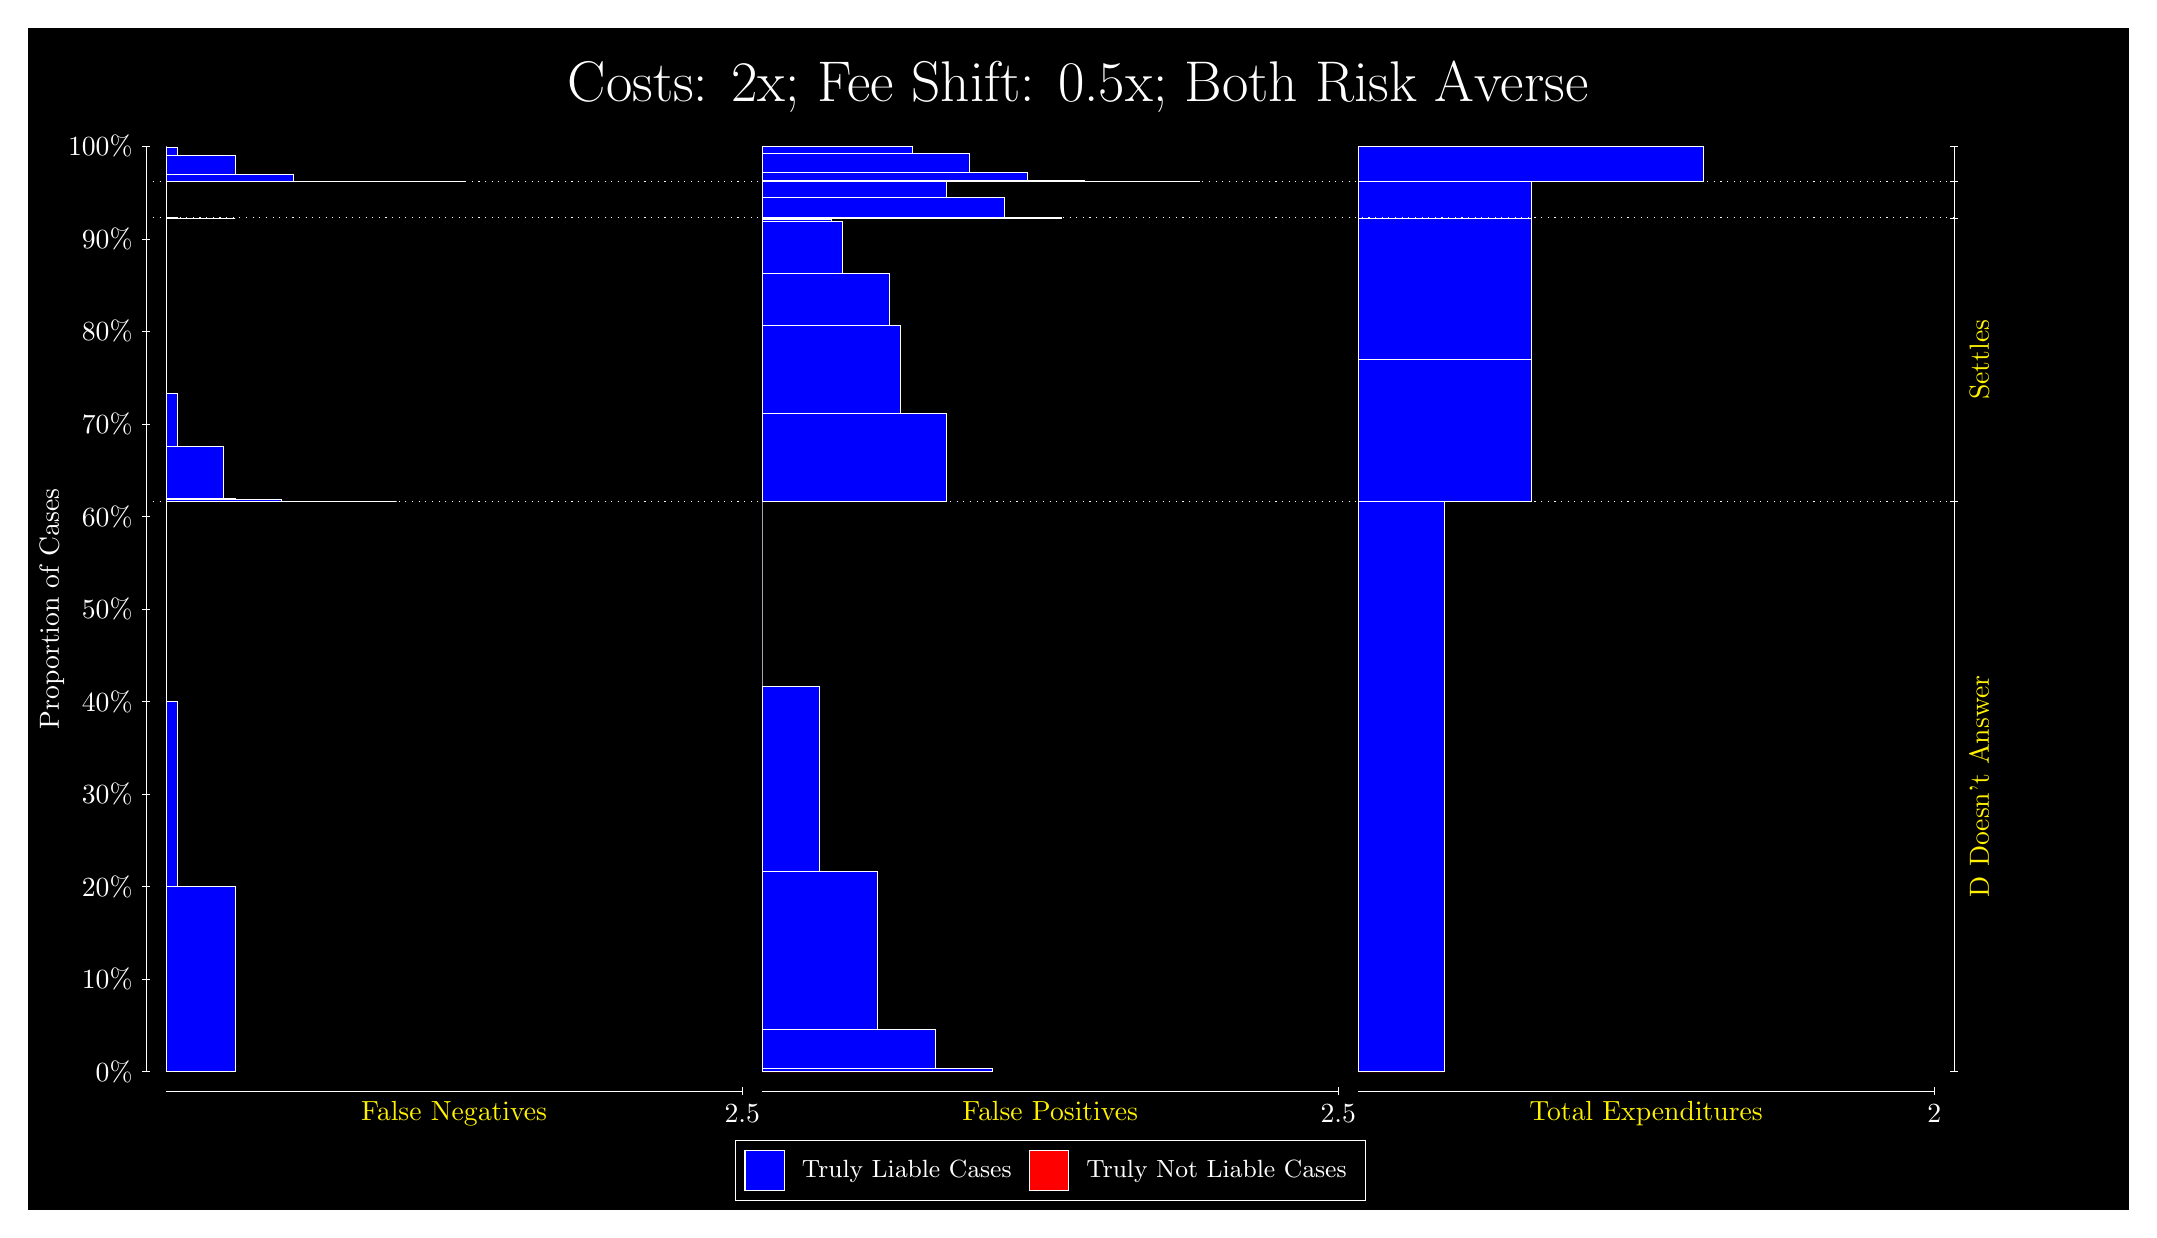
\begin{tikzpicture}
\draw[fill=black] (0,0) rectangle (26.667,15);
\draw[text=white] (0,13.5) rectangle (26.667,15) node[midway] {\huge Costs: 2x; Fee Shift: 0.5x; Both Risk Averse};
\draw[white, very thin] (1.5,1.75) -- (1.5,13.5);
\node[rotate=90, text=white, anchor=center] at (0.3, 7.625) {Proportion of Cases};
\draw[white, very thin] (1.45,1.75) -- (1.55,1.75);
\node[text=white, anchor=east] at (1.45, 1.75) {0\%};
\draw[white, very thin] (1.45,2.925) -- (1.55,2.925);
\node[text=white, anchor=east] at (1.45, 2.925) {10\%};
\draw[white, very thin] (1.45,4.1) -- (1.55,4.1);
\node[text=white, anchor=east] at (1.45, 4.1) {20\%};
\draw[white, very thin] (1.45,5.275) -- (1.55,5.275);
\node[text=white, anchor=east] at (1.45, 5.275) {30\%};
\draw[white, very thin] (1.45,6.45) -- (1.55,6.45);
\node[text=white, anchor=east] at (1.45, 6.45) {40\%};
\draw[white, very thin] (1.45,7.625) -- (1.55,7.625);
\node[text=white, anchor=east] at (1.45, 7.625) {50\%};
\draw[white, very thin] (1.45,8.8) -- (1.55,8.8);
\node[text=white, anchor=east] at (1.45, 8.8) {60\%};
\draw[white, very thin] (1.45,9.975) -- (1.55,9.975);
\node[text=white, anchor=east] at (1.45, 9.975) {70\%};
\draw[white, very thin] (1.45,11.15) -- (1.55,11.15);
\node[text=white, anchor=east] at (1.45, 11.15) {80\%};
\draw[white, very thin] (1.45,12.325) -- (1.55,12.325);
\node[text=white, anchor=east] at (1.45, 12.325) {90\%};
\draw[white, very thin] (1.45,13.5) -- (1.55,13.5);
\node[text=white, anchor=east] at (1.45, 13.5) {100\%};

\draw[white, very thin] (24.457,1.75) -- (24.457,13.5);
\draw[white, very thin] (24.407,1.75) -- (24.507,1.75);
\node[anchor=west] at (24.407, 1.75) {};
\draw[white, very thin] (24.407,8.9913) -- (24.507,8.9913);
\node[anchor=west] at (24.407, 8.9913) {};
\draw[white, very thin] (24.407,12.591) -- (24.507,12.591);
\node[anchor=west] at (24.407, 12.591) {};
\draw[white, very thin] (24.407,13.056) -- (24.507,13.056);
\node[anchor=west] at (24.407, 13.056) {};
\draw[white, very thin] (24.407,13.5) -- (24.507,13.5);
\node[anchor=west] at (24.407, 13.5) {};

\draw[white, very thin, fill=blue] (1.75,1.75) rectangle (2.6283,4.0999);
\draw[white, very thin, fill=blue] (1.75,4.0999) rectangle (1.8964,6.447);
\draw[white, very thin, fill=red] (1.75,6.447) rectangle (1.75,6.447);
\draw[white, very thin, fill=blue] (1.75,6.447) rectangle (1.75,8.9913);
\draw[white, very thin, fill=blue] (1.75,8.9913) rectangle (4.6775,8.9913);
\draw[white, very thin, fill=blue] (1.75,8.9913) rectangle (4.092,8.9913);
\draw[white, very thin, fill=blue] (1.75,8.9913) rectangle (3.9457,8.9913);
\draw[white, very thin, fill=blue] (1.75,8.9913) rectangle (3.3602,8.9913);
\draw[white, very thin, fill=blue] (1.75,8.9913) rectangle (3.2138,9.0133);
\draw[white, very thin, fill=blue] (1.75,9.0133) rectangle (2.6283,9.0359);
\draw[white, very thin, fill=blue] (1.75,9.0359) rectangle (2.4819,9.6936);
\draw[white, very thin, fill=blue] (1.75,9.6936) rectangle (1.8964,10.361);
\draw[white, very thin, fill=red] (1.75,10.361) rectangle (1.75,10.361);
\draw[white, very thin, fill=blue] (1.75,10.361) rectangle (1.75,12.591);
\draw[white, very thin, fill=blue] (1.75,12.591) rectangle (2.6283,12.591);
\draw[white, very thin, fill=blue] (1.75,12.591) rectangle (1.8964,12.593);
\draw[white, very thin, fill=red] (1.75,12.593) rectangle (1.75,12.593);
\draw[white, very thin, fill=blue] (1.75,12.593) rectangle (1.75,13.056);
\draw[white, very thin, fill=blue] (1.75,13.056) rectangle (5.5558,13.056);
\draw[white, very thin, fill=blue] (1.75,13.056) rectangle (4.8239,13.056);
\draw[white, very thin, fill=blue] (1.75,13.056) rectangle (4.092,13.058);
\draw[white, very thin, fill=blue] (1.75,13.058) rectangle (3.3602,13.145);
\draw[white, very thin, fill=blue] (1.75,13.145) rectangle (2.6283,13.145);
\draw[white, very thin, fill=blue] (1.75,13.145) rectangle (2.6283,13.38);
\draw[white, very thin, fill=blue] (1.75,13.38) rectangle (1.8964,13.38);
\draw[white, very thin, fill=blue] (1.75,13.38) rectangle (1.8964,13.489);
\draw[white, very thin, fill=red] (1.75,13.489) rectangle (1.75,13.489);
\draw[white, very thin, fill=blue] (1.75,13.489) rectangle (1.75,13.5);
\draw[white, very thin, fill=red] (9.3189,1.75) rectangle (12.246,1.75);
\draw[white, very thin, fill=blue] (9.3189,1.75) rectangle (12.246,1.7883);
\draw[white, very thin, fill=blue] (9.3189,1.7883) rectangle (11.515,2.288);
\draw[white, very thin, fill=blue] (9.3189,2.288) rectangle (10.783,4.2943);
\draw[white, very thin, fill=blue] (9.3189,4.2943) rectangle (10.051,6.6414);
\draw[white, very thin, fill=blue] (9.3189,6.6414) rectangle (9.3189,8.9913);
\draw[white, very thin, fill=red] (9.3189,8.9913) rectangle (11.661,8.9913);
\draw[white, very thin, fill=blue] (9.3189,8.9913) rectangle (11.661,10.107);
\draw[white, very thin, fill=red] (9.3189,10.107) rectangle (11.075,10.107);
\draw[white, very thin, fill=blue] (9.3189,10.107) rectangle (11.075,11.222);
\draw[white, very thin, fill=blue] (9.3189,11.222) rectangle (10.929,11.889);
\draw[white, very thin, fill=blue] (9.3189,11.889) rectangle (10.344,12.547);
\draw[white, very thin, fill=blue] (9.3189,12.547) rectangle (10.197,12.569);
\draw[white, very thin, fill=blue] (9.3189,12.569) rectangle (9.6116,12.591);
\draw[white, very thin, fill=blue] (9.3189,12.591) rectangle (9.4652,12.591);
\draw[white, very thin, fill=blue] (9.3189,12.591) rectangle (9.3189,12.591);
\draw[white, very thin, fill=red] (9.3189,12.591) rectangle (13.125,12.591);
\draw[white, very thin, fill=blue] (9.3189,12.591) rectangle (13.125,12.599);
\draw[white, very thin, fill=blue] (9.3189,12.599) rectangle (12.393,12.857);
\draw[white, very thin, fill=blue] (9.3189,12.857) rectangle (11.661,13.054);
\draw[white, very thin, fill=blue] (9.3189,13.054) rectangle (10.929,13.056);
\draw[white, very thin, fill=blue] (9.3189,13.056) rectangle (10.197,13.056);
\draw[white, very thin, fill=red] (9.3189,13.056) rectangle (14.881,13.056);
\draw[white, very thin, fill=blue] (9.3189,13.056) rectangle (14.881,13.056);
\draw[white, very thin, fill=red] (9.3189,13.056) rectangle (14.149,13.056);
\draw[white, very thin, fill=blue] (9.3189,13.056) rectangle (14.149,13.056);
\draw[white, very thin, fill=red] (9.3189,13.056) rectangle (13.417,13.056);
\draw[white, very thin, fill=blue] (9.3189,13.056) rectangle (13.417,13.067);
\draw[white, very thin, fill=red] (9.3189,13.067) rectangle (12.686,13.067);
\draw[white, very thin, fill=blue] (9.3189,13.067) rectangle (12.686,13.176);
\draw[white, very thin, fill=red] (9.3189,13.176) rectangle (11.954,13.176);
\draw[white, very thin, fill=blue] (9.3189,13.176) rectangle (11.954,13.411);
\draw[white, very thin, fill=blue] (9.3189,13.411) rectangle (11.222,13.498);
\draw[white, very thin, fill=blue] (9.3189,13.498) rectangle (10.49,13.5);
\draw[white, very thin, fill=blue] (9.3189,13.5) rectangle (9.758,13.5);
\draw[white, very thin, fill=blue] (9.3189,13.5) rectangle (9.3189,13.5);
\draw[white, very thin, fill=red] (16.888,1.75) rectangle (17.986,1.75);
\draw[white, very thin, fill=blue] (16.888,1.75) rectangle (17.986,8.9913);
\draw[white, very thin, fill=red] (16.888,8.9913) rectangle (19.083,8.9913);
\draw[white, very thin, fill=blue] (16.888,8.9913) rectangle (19.083,10.796);
\draw[white, very thin, fill=red] (16.888,10.796) rectangle (19.083,10.796);
\draw[white, very thin, fill=blue] (16.888,10.796) rectangle (19.083,12.591);
\draw[white, very thin, fill=red] (16.888,12.591) rectangle (19.083,12.591);
\draw[white, very thin, fill=blue] (16.888,12.591) rectangle (19.083,13.056);
\draw[white, very thin, fill=red] (16.888,13.056) rectangle (21.279,13.056);
\draw[white, very thin, fill=blue] (16.888,13.056) rectangle (21.279,13.5);
\draw[white, dotted] (1.5,8.9913) -- (24.457,8.9913);
\draw[white, dotted] (1.5,12.591) -- (24.457,12.591);
\draw[white, dotted] (1.5,13.056) -- (24.457,13.056);
\draw[white, very thin] (1.75,1.5) -- (9.0689,1.5);
\node[text=yellow, anchor=north] at (5.4094, 1.5) {False Negatives};
\draw[white, very thin] (9.0689,1.45) -- (9.0689,1.55);
\node[text=white, anchor=north] at (9.0689, 1.45) {2.5};

\draw[white, very thin] (9.3189,1.5) -- (16.638,1.5);
\node[text=yellow, anchor=north] at (12.978, 1.5) {False Positives};
\draw[white, very thin] (16.638,1.45) -- (16.638,1.55);
\node[text=white, anchor=north] at (16.638, 1.45) {2.5};

\draw[white, very thin] (16.888,1.5) -- (24.207,1.5);
\node[text=yellow, anchor=north] at (20.547, 1.5) {Total Expenditures};
\draw[white, very thin] (24.207,1.45) -- (24.207,1.55);
\node[text=white, anchor=north] at (24.207, 1.45) {2};

\node[text=yellow, centered, rotate=90] at (24.777, 5.3706) {D Doesn't Answer};
\node[text=yellow, centered, rotate=90] at (24.777, 10.791) {Settles};



\draw (12.978300999999998,1.5) node[draw=none] (baseCoordinate) {};
\begin{scope}[align=center]
        \matrix[scale=0.5, draw=white, below=0.5cm of baseCoordinate, nodes={draw}, column sep=0.1cm]{
            \node[rectangle, draw, minimum width=0.5cm, minimum height=0.5cm, fill=blue] {}; &
            \node[draw=none, font=\small, text=white] (B) {Truly Liable Cases}; &
            \node[rectangle, draw, minimum width=0.5cm, minimum height=0.5cm, fill=red] {}; &
            \node[draw=none, font=\small, text=white] (B) {Truly Not Liable Cases}; \\
            };
\end{scope}

\end{tikzpicture}
\end{document}